% !TeX spellcheck = en_GB
\documentclass[letterpaper,12pt]{article}
\usepackage{textcomp}
\usepackage{parskip}
\usepackage{amsmath}
\usepackage{amssymb}
\usepackage{mathrsfs}
\usepackage{gensymb}
\usepackage{enumerate}
\usepackage{fullpage}
\usepackage{setspace}
\usepackage{array}
\usepackage{threeparttable}
\usepackage{graphicx}
\usepackage{float}

\onehalfspacing

\setlength{\parindent}{0pt}
\newcommand{\vect}[1]{\mathbf{#1}}
\newcommand*\conj[1]{\bar{#1}}
\setlength{\belowcaptionskip}{-80pt}


\begin{document}

\textbf{\large Problem Set 5}

Natasha Watkins

\vspace{5mm}

\textbf{Exercise 8.1}
\begin{figure}[H]
	\centering
	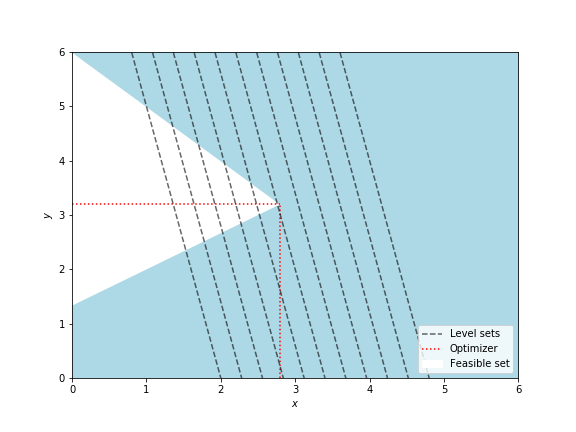
\includegraphics[scale=0.45]{plot1.png}
	\label{plot1}
\end{figure}
The optimizer is (2.8, 3.2).

\textbf{Exercise 8.2}

\underline{Part i)}
\begin{figure}[H]
	\centering
	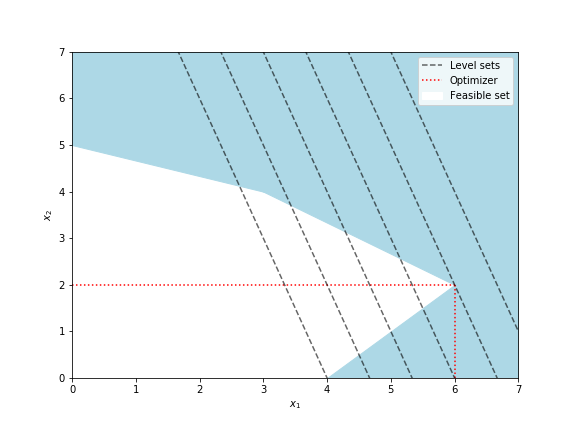
\includegraphics[scale=0.45]{plot2.png}
	\label{plot1}
\end{figure}
The optimizer is (6, 2).

\underline{Part ii)}
\begin{figure}[H]
	\centering
	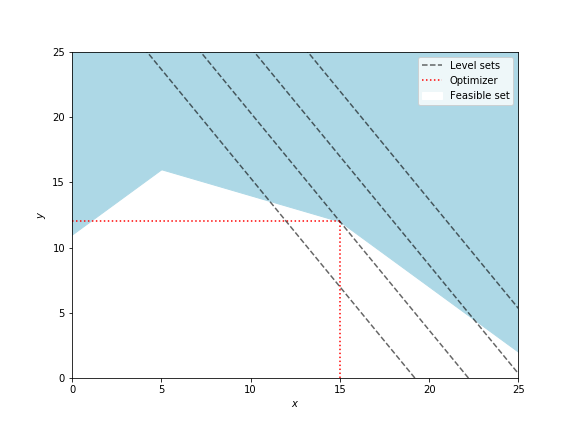
\includegraphics[scale=0.45]{plot3.png}
	\label{plot1}
\end{figure}
The optimizer is (15, 12).

\textbf{Exercise 8.3}

$x_1$ is a GI Barb soldier, $x_2$ is a Joey doll. The optimisation problem is
\begin{align*}
\max_{x_1, x_2} \ & 4x_1 + 3x_2 \\
\text{s. t.} \quad & x_2 \leq 200 \\
& 15x_1 + 10 x_2 \leq 1800 \\
& 2x_1 + 2x_2 \leq 300 \\
& x_1, x_2 \geq 0
\end{align*}

\textbf{Exercise 8.4}

The optimisation problem is
\begin{align*}
\min{_{x_{ij}}} \quad & 2 x_{AB} + 5 x_{BC} + 2 x_{CF} + 9 x_{BF} + 3 x_{EF} + 7 x_{BE} + 2 x_{BD} + 4 x_{DE} + 5 x_{AD} + 2 x_{BD} \\
\text{s. t.} \quad & x_{AD} + x_{AB} = 10 \\
& -x_{AB} + x_{BC} + x_{BF} + x_{BE} + x_{BD} = 1 \\
& -x_{BC} + x_{CF} = -2 \\
& -x_{AD} - x_{BD} + x_{DE} = -3 \\
& -x_{DE} - x_{BE} + x_{EF} = 4 \\
& -x_{EF} - x_{BF} - x_{CF} = -10 \\
& 0 \leq x_{i, j} \leq 6
\end{align*}

\textbf{Exercise 8.5}

* Dictionaries adapted from Reiko's code.

\underline{Part i)}

\begin{center}
	$\begin{array}{ c c c c c c c c  }
		\zeta & = & & & 3x_1 & + & x_2 \\
		\hline
		w_1 & = & 15 & - & x_1 & - & 3x_2 \\
		w_2 & = & 18 & - & 2x_1 & - & 3x_2 \\
		w_3 & = & 4 & - & x_1 & + & x_2 \\
	\end{array}$ \\
\end{center}

$w_3$ is binding, so we increase $x_1$ by 4. \\

\begin{center}
	$\begin{array}{ c c c c c c c c  }
		\zeta & = & 12 & + & 4x_2 & - & 3w_3 \\
		\hline
		w_1 & = & 11 & - & 4x_2 & + & w_3 \\
		w_2 & = & 10 & - & 5x_2 & + & 2w_3 \\
		x_1 & = & 4 & + & x_2 & - & w_3 \\
	\end{array}$ \\
\end{center}

$w_2$ is binding, so we increase $x_2$ by 2. \\

\begin{center}
	$\begin{array}{ c c c c c c c c  }
		\zeta & = & 20 & - & \tfrac{4}{5}w_2 & - & \tfrac{7}{5}w_3 \\
		\hline
		w_1 & = & 3 & + & \tfrac{4}{5}w_2 & - & \tfrac{3}{5}w_3 \\
		x_2 & = & 2 & - & \tfrac{1}{5}w_2 & + & \tfrac{2}{5}w_3 \\
		x_1 & = & 6 & - & \tfrac{1}{5}w_2 & - & \tfrac{3}{5}w_3\\
	\end{array}$
\end{center}

We can no longer increase the variables in the objective function, so the optimum value of the objective function is 20 and the optimal point is (6, 2).

\underline{Part ii)}


\begin{center}
	$\begin{array}{ c c c c c c c c  }
	\zeta & = & & & 4x & + & 6y \\
	\hline
	w_1 & = & 11 & + & x & - & y \\
	w_2 & = & 27 & - & x & - & y \\
	w_3 & = & 90 & - & 2x & - & 5y \\
	\end{array}$ \\
\end{center}

$w_2$ is binding, so we increase $x$ by 27. \\

\begin{center}
	$\begin{array}{ c c c c c c c c  }
	\zeta & = & 108 & - & 4w_2 & + & 2y \\
	\hline
	w_1 & = & 38 & - & w_2 & - & 2y \\
	x & = & 27 & - & w_2 & + & y \\
	w_1 & = & 26 & - & 2w_2 & - & 3y \\
	\end{array}$ \\
\end{center}

$w_3$ is binding, so we increase $y$ by 12. \\

\begin{center}
	$\begin{array}{ c c c c c c c c  }
	\zeta & = & 132 & - & \tfrac{16}{3}w_2 & - & \tfrac{2}{3}w_3 \\
	\hline
	w_1 & = & 14 & + & \tfrac{7}{3}w_2 & - & \tfrac{2}{3}w_3 \\
	x & = & 15 & - & \tfrac{5}{3}w_2 & - & \tfrac{1}{3}w_3 \\
	y & = & 12 & - & \tfrac{2}{3}w_2 & - & \tfrac{1}{3}w_3\\
	\end{array}$
\end{center}

We can no longer increase the variables in the objective function, so the optimum value of the objective function is 132 and the optimal point is (15, 12).

\textbf{Exercise 8.6}


\begin{center}
	$\begin{array}{ c c c c c c c c  }
	\zeta & = & & & 4x_1 & + & 3x_2 \\
	\hline
	w_1 & = & 200 & & & - & x_2 \\
	w_2 & = & 360 & - & 3x_1 & - & 2x_2 \\
	w_3 & = & 150 & - & x_1 & - & x_2 \\
	\end{array}$ \\
\end{center}

$w_2$ is binding, so we increase $x_1$ by 120. \\

\begin{center}
	$\begin{array}{ c c c c c c c c  }
	\zeta & = & 480 & - & \frac{4}{3}w_2 & + & \frac{1}{3}x_2 \\
	\hline
	w_1 & = & 200 & & & - & x_2 \\
	x_1 & = & 120 & - & \frac{1}{3}w_2 & - & \frac{2}{3}x_2 \\
	w_3 & = & 30 & + & \frac{1}{3}w_2 & - & \frac{1}{3}x_2 \\
	\end{array}$ \\
\end{center}

$w_3$ is binding, so we increase $x_2$ by 90. \\

\begin{center}
	$\begin{array}{ c c c c c c c c  }
	\zeta & = & 510 & - & w_2 & - & \frac{1}{3}w_3 \\
	\hline
	w_1 & = & 110 & - & w_2 & + & w_3 \\
	x_1 & = & 60 & - & w_2 & - & \frac{2}{3}w_3 \\
	x_2 & = & 90 & + & w_2 & - & w_3 \\
	\end{array}$ \\
\end{center}

We can no longer increase the variables in the objective function, so the maximum profit \$510 with supply of 60 GI Barb toys and 90 Joey dolls.

\textbf{Exercise 8.7}

\underline{Part i)}

As one of the constraints has a negative constant, the origin is infeasible. We will first need to solve the auxiliary problem, given as
\begin{center}
	$\begin{array}{ c c c c c c c c c c }
	\zeta & = &  &   &      &   &      &   & -x_o \\
	\hline
	w_1 & = & -8 & + & 4x_1 & + & 2x_2 & + & x_0 \\
	w_2 & = & 6  & + & 2x_1 & - & 3x_2 & + & x_0 \\
	w_3 & = & 3  & - & x_1  &   &      & + & x_0 \\
	\end{array}$ \\
\end{center}

This problem is infeasible. We will pivot with $w_1$, the most negative constraint.
\begin{center}
	$\begin{array}{ c c c c c c c c c c }
	\zeta & = & -8 &  + & 4x_1 & + & 2x_2 & - & w_1 \\
	\hline
	x_0 & = & 8 & - & 4x_1 & - & 2x_2 & + & w_1 \\
	w_2 & = & 14  & - & 2x_1 & - & 5x_2 & + & w_1 \\
	w_3 & = & 11  & - & 5x_1  & -  &  2x_2 & + & w_1 \\
	\end{array}$ \\
\end{center}

We need the objective function of the auxiliary problem to be 0, so we will pivot $x_1$ with its binding constraint $x_0$.
\begin{center}
	$\begin{array}{ c c c c c c c c c c }
	\zeta & = &  &   &      &   &      &   & -x_o \\
	\hline
	x_1 & = & 2 & + & \frac{1}{2}w_1 & - & \frac{1}{2}x_2 & - & \frac{1}{4}x_0 \\
	w_2 & = & 10  & + & \frac{1}{2}w_1 & - & 4x_2 & + & \frac{1}{2}x_0 \\
	w_3 & = & 1  & - & \frac{1}{4}w_0  & +  &  \frac{1}{2}x_2 & + & \frac{5}{4}x_0 \\
	\end{array}$ \\
\end{center}

\underline{Part ii)}

As one of the constraints has a negative constant, the origin is infeasible. We will first need to solve the auxiliary problem, given as
\begin{center}
	$\begin{array}{ c c c c c c c c c c }
	\zeta & = &  &   &      &   &      &   & -x_o \\
	\hline
	w_1 & = & 15 & - & 5x_1 & - & 3x_2 & + & x_0 \\
	w_2 & = & 15  & - & 3x_1 & - & 5x_2 & + & x_0 \\
	w_3 & = & -12  & - & 4x_1  & + &  3x_1 & + & x_0 \\
	\end{array}$ \\
\end{center}

This problem is infeasible. We will pivot with $w_3$, the most negative constraint.
\begin{center}
	$\begin{array}{ c c c c c c c c c c }
	\zeta & = & -12 & - & 4x_1 & + & 3x_2 & - & w_1 \\
	\hline
	w_1 & = & 27 & - & x_1 & - & 6x_2 & + & w_1 \\
	w_2 & = & 12  & - & x_1 & - & 8x_2 & + & w_1 \\
	x_0 & = & 12  & + & 4x_1  & -  &  3x_2 & + & w_1 \\
	\end{array}$ \\
\end{center}

We need the objective function of the auxiliary problem to be 0, so we will pivot $x_2$ with its binding constraint $w_2$.
\begin{center}
	$\begin{array}{ c c c c c c c c c c }
	\zeta & = & -\frac{15}{8} & - & \frac{29}{8}x_1 & - & \frac{3}{8}w_1 & - & \frac{5}{8}w_2 \\
	\hline
	w_1 & = & \frac{27}{4} & - & \frac{7}{4}x_1 & + & \frac{3}{4}w_1 & + & \frac{1}{4}w_2 \\
	x_2 & = & \frac{27}{8}  & + & \frac{1}{8}x_1 & - & \frac{1}{8}w_1 & + & \frac{1}{8}w_2 \\
	x_0 & = & \frac{15}{8}  & + & \frac{29}{8}x_1  & +  &  \frac{3}{8}w_1 & + & \frac{5}{8}w_2 \\
	\end{array}$ \\
\end{center}
As the value of the objective function is negative, the original problem is infeasible.

\underline{Part iii)}

\begin{center}
	$\begin{array}{ c c c c c c c c  }
	\zeta & = & & & -3x_1 & + & x_2 \\
	\hline
	w_1 & = & 4 & & & - & x_2 \\
	w_2 & = & 6 & + & 2x_1 & - & 3x_2 \\
	\end{array}$ \\
\end{center}

We can only increase $x_2$. The binding constraint is $w_2$, so we increase $x_2$ by 2.

\begin{center}
 	$\begin{array}{ c c c c c c c c  }
 	\zeta & = & 2 & - & 2x_1 & - & \frac{1}{3}w_2 \\
 	\hline
 	w_1 & = & 2 & - & x_1 & + & \frac{1}{3}w_2 \\
 	x_2 & = & 2 & + & x_1 & - & \frac{1}{3}w_2 \\
 	\end{array}$ \\
\end{center}

The optimal value is therefore 2 at (0, 2).

\textbf{Exercise 8.15}

We have $A \vect{x} \leq \vect{b}$ and $A^T \vect{y} \geq \vect{c}$.
\begin{align*}
A \vect{x} &\leq \vect{b} \\
\vect{x}^T A^T &\leq \vect{b}^T \\
\vect{x}^T A^T \vect{y} &\leq \vect{b}^T \vect{y} \\
\vect{x}^T \vect{c} &\leq \vect{b}^T \vect{y} \\
\vect{c}^T \vect{x} &\leq \vect{b}^T \vect{y} \quad \text{as } {\vect{c}^T \vect{x}} \text{ is scalar}\\
\end{align*}

\textbf{Exercise 8.17}

Consider the primal problem
\begin{align*}
\max \ & \vect{c}^T \vect{x} \\
\text{s.t.} \ & A \vect{x} \preceq \vect{b} \\
& \vect{x} \preceq \vect{0}
\end{align*}
With the dual problem
\begin{align*}
\min \ & \vect{b}^T \vect{y} \\
\text{s.t.} \ & A^T \vect{y} \succeq \vect{c} \\
& \vect{y} \succeq \vect{0}
\end{align*}
This is equivalent to
\begin{align*}
\max \ & \vect{-b}^T \vect{y} \\
\text{s.t.} \ & -A^T \vect{y} \preceq -\vect{c} \\
& \vect{y} \succeq \vect{0}
\end{align*}
Taking the dual of this, we have
\begin{align*}
\min \ & \vect{-c}^T \vect{x} \\
\text{s.t.} \ & -(A^T)^T \vect{x} \succeq -\vect{b} \\
& \vect{x} \succeq \vect{0}
\end{align*}
which is equivalent to the primal problem.

\textbf{Exercise 8.18}

Solving the primal problem...
\begin{center}
	$\begin{array}{ c c c c c c c c  }
	\zeta & = & & & x_1 & + & x_2 \\
	\hline
	w_1 & = & 3 & - & 2x_1 & - & x_2 \\
	w_2 & = & 5 & - & x_1 & - & 3x_2 \\
	w_3 & = & 4 & - & 2x_1 & - & 3x_2 \\
	\end{array}$ \\
\end{center}

If we increase $x_1$, $w_1$ is binding. \\

\begin{center}
	$\begin{array}{ c c c c c c c c  }
	\zeta & = & \frac{3}{2} & - & \frac{1}{2}w_1 & + & \frac{1}{2}x_2 \\
	\hline
	x_1 & = & \frac{3}{2} & - & \frac{1}{2}w_1 & - & \frac{1}{2}x_2 \\
	w_2 & = & \frac{7}{2} & - & \frac{1}{2}w_1 & - & \frac{5}{2}x_2 \\
	w_3 & = & 1 & + & w_1 & - & 2x_2 \\
	\end{array}$ \\
\end{center}

If we increase $x_2$, $w_3$ is binding. \\

\begin{center}
	$\begin{array}{ c c c c c c c c  }
	\zeta & = & \frac{7}{4} & - & \frac{1}{4}w_1 & - & \frac{1}{4}w_2 \\
	\hline
	x_1 & = & \frac{5}{4} & - & \frac{3}{2}w_1 & + & \frac{1}{4}w_3 \\
	w_2 & = & \frac{9}{4} & - & \frac{3}{4}w_1 & + & \frac{5}{4}w_3 \\
	x_2 & = & \frac{1}{2} & + & \frac{1}{2}w_1 & - & \frac{1}{2}w_3 \\
	\end{array}$ \\
\end{center}

We can no longer increase the variables in the objective function, so the optimum value of the objective function is $\frac{7}{4}$ and the optimal point is $(\frac{5}{4}, \frac{1}{2})$.

The dual problem is
\begin{align*}
\min_{y_1, y_2, y_3} & 3y_1 + 5y_2 + 4y_3 \\
\text{s.t.} \ & 2y_1 + y_2 + 2y_3 \geq 1 \\
&y_1 + 3 y_2 + 3y_3 \geq 1 \\
& y_1, y_2, y_3 \geq 0
\end{align*}

\end{document}